\chapter{Solution}

\section{Introduction}

Taking requirements into consideration, desired platform clearly has features common to a autonomic system, especially the need for automatic environment reconfiguration. One of the first architectures that satisfied that requirement was proposed by \cite{IBM06}. Beside this, system under consideration has a character of a multi-layered one (i.e. it operates on a application / container / service / cloud level). Optimally, each level should be characterized by different actions, what can be meet by implementing multi-hierarchical autonomic system, as proposed in \cite{LiWoZh05}.

Considering that observation, auto-scaling subsystem spans across different layers:

\begin{figure}[!ht]
  \begin{center}
    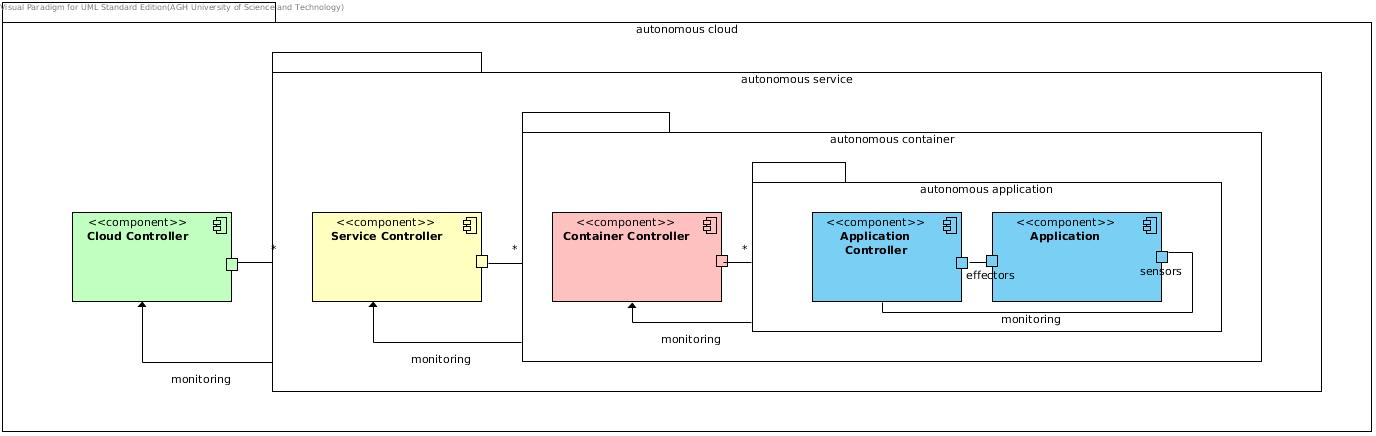
\includegraphics[width=\textwidth]{chapter-5/hierarchical-autonomic-system}
  \end{center}
  \caption{Hierarchical autonomic system}
  \label{ch5:hierarchical-autonomic-system}
\end{figure}

Remaining of this section breaks apart each functional module of an autonomic component, whereas further sections cover in details each autonomic level.

\subsection{Autonomic component}

\begin{figure}[!ht]
  \begin{center}
    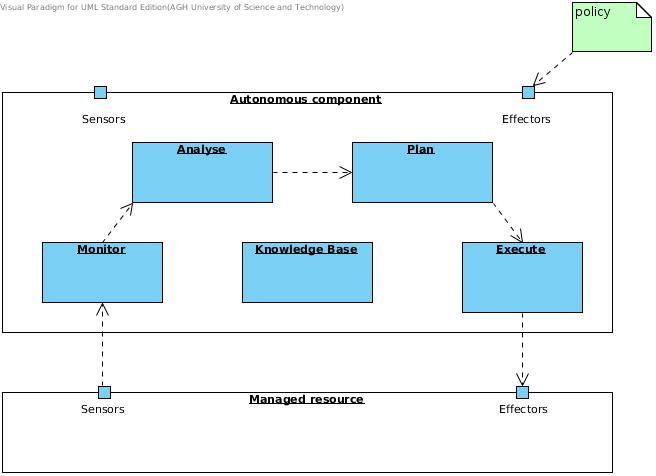
\includegraphics[width=0.8\textwidth]{chapter-5/autnomic-component}
  \end{center}
  \caption{Autonomic component}
  \label{ch5:autonomic-component}
\end{figure}

\subsubsection{Monitor}

Monitor module is responsible for gathering monitoring data from \textit{Sensors} and store them in a database, correlated with a specific autonomous component (ie. application / container / service / cloud). Problem of a multi-layered, hierarchical self-adaptive monitoring system is described in \cite{KaKoGoKyMeVa12}.


\subsubsection{Analyse}

Analyse module performs analysis of a gathered data. There is a variety of models that helps to achieve this goal. For example, the \cite{LiWoZh05} proposes:

\begin{itemize}
	\item Queue-based Performance Models
	\item Dynamic models
	\item Monotonic static models
	\item Policy based models
\end{itemize}

Details about which level leverage which model are presented in detailed architecture description. Important part in a data analysis plays a predictive approach \cite{JiPeLiCh11} and tracking changes in a system \cite{ZhYaWo05}.

\subsubsection{Plan}

This module is responsible for scheduling actions that have to be taken to solve problems reported by an earlier analysis. This may involve:
\begin{itemize}
	\item reserving some resources (for example to deploy a new virtual machine)
	\item handling situation where multiple entities compete about the resources (for example by a prioritization)
\end{itemize}

It is possible, however, that resolving issues is not possible at current level. It that case, the upper-level is responsible for handling it.

\subsubsection{Execute}

Execute module is directly responsible for managing resource, by performing various operations on resource's effector. Each layer is characterized by different actions that can be taken, for example: application server reconfiguration, vertical or horizontal scaling.

\subsubsection{Knowledge base}

Knowledge base is represented as a set of rules, policies shared across autonomous components.

\subsection{Managed resource}

\subsubsection{Effector}

Enables management of a resources by exposing some API compatible with an Executor.

\subsubsection{Sensor}

Aim of a sensor is probing a resource and sending back results to a Monitor. There are different kind of metrics that should be considered such as: CPU load, memory usage or response delay.



\section{Application controller}

\section{Container controller}

\section{Service controller}

\section{Cloud controller}